\newpage

\section{Theoretical Analysis}
\label{sec:analysis}

\subsection{Central Frequency, Voltage Gain, Input and Output impedances}
Octave was used to compute the following values: central frequency, voltage gain, input impedance and output impedance. \par
The following equations were given by the professor:
\begin{equation}
    T(s) = \frac{R_1 C_1 s}{1+ R_1 C_1 s} (1+\frac{R_3}{R_4}) \frac{1}{1+ R_2 C_2 s}
\end{equation}\par
 \par
\begin{equation}
    Lower_{cutoff} = \frac{1}{R_1 C_1}
\end{equation}\par
and \par
\begin{equation}
    Upper_{cutoff} = \frac{1}{R_2 C_2}
\end{equation}\par
The Octave values are in the table below:

\begin{center}
  \begin{tabular}{ | c | c | }
    \hline    
    {\bf Name} & {\bf Value [$Hz$, $dB$ or $\Omega$]} \\ \hline
    Central Frequency & 5.603677e+02 \\ \hline 
Voltage Gain dB & 5.156477e+01 \\ \hline 
Input Impedance & 5.000000e+02 \\ \hline 
Output Impedance & 4.347826e+02 \\ 

    \hline
  \end{tabular}
  \captionof{figure}{Central Frequency, Voltage Gain, Input and Output impedances}
\end{center}

\subsection{Frequency Response}
Frequency response is ploted in in $dB$ as shown:\par

\begin{figure}[H] \centering
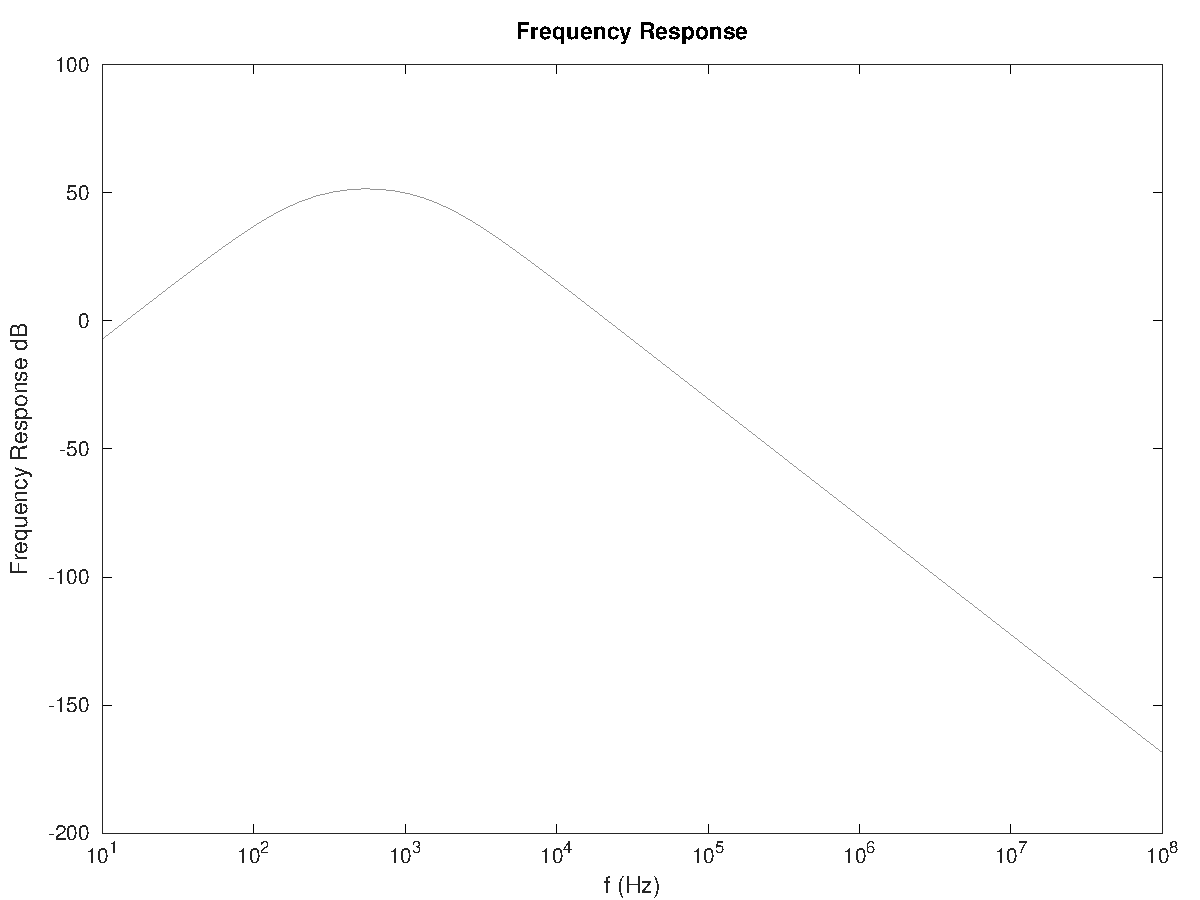
\includegraphics[width=0.7\linewidth]{../mat/fresponse1.pdf}
\caption{Frequency Response - $dB$}
\label{fig:fresponse1}
\end{figure}


\begin{figure}[H] \centering
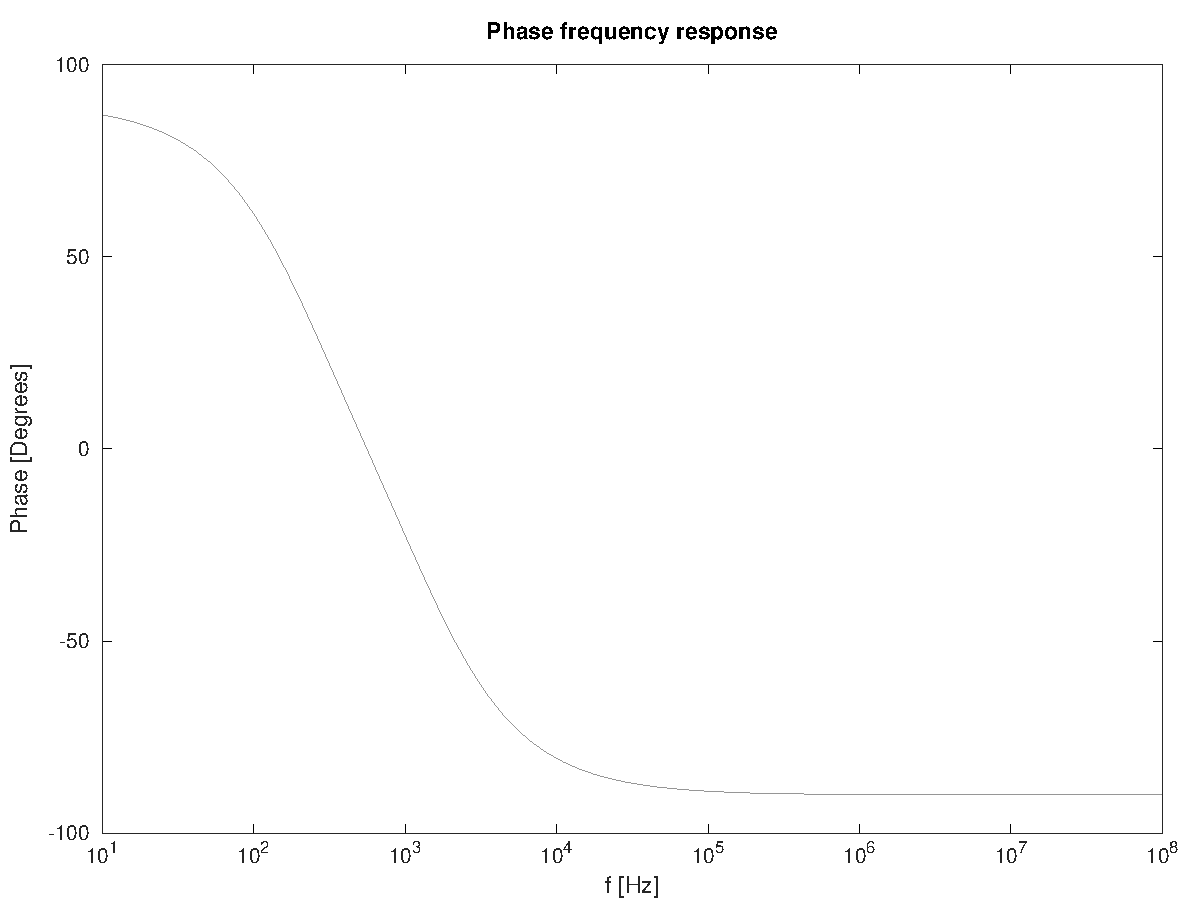
\includegraphics[width=0.7\linewidth]{../mat/fresponse2.pdf}
\caption{Frequency Response - Phase}
\label{fig:fresponse2}
\end{figure}